%%%%%%%%%%%%%%%%%%%%%%%%%%%%%%%%%%%%%%%%%%%%%%%%%
%
%     Chapter 6
%
%%%%%%%%%%%%%%%%%%%%%%%%%%%%%%%%%%%%%%%%%%%%%%%%

\chapter{Performance Evaluation}
\label{six}

In this chapter, we focus on the performance evaluation to assess whether our LLVM back end matches the performance of the hand-written library and whether back end optimizations provide performance advantages. We first validate our vector of $i2^k$ approaches, and then present the performance of some critical Parabix operations via an application-level profile.

\section{Vector of $i2^k$ Performance}
In Chapter~\ref{four}, we presented different approaches to lower $i1$, $i2$, $i4$ and some $i8$ operations within one SIMD register. In this section, we validate our approaches by showing the improved run-time performance.

\subsection{Methodology}

Testing small pieces of critical code can be tricky, since the testing overhead can easily overwhelm the critical code and make the result meaningless. Agner Fog provides a test program which uses the Time Stamp Counter for clock cycles and Performance Monitor Counters for instruction count and other related events \cite{agner_testp}. We measure the reciprocal throughput, the CPU cycles and the instructions count. The reciprocal throughput is measured with a sequence of same instructions where subsequent instructions are independent of the previous ones. In Fog's instruction table, he noted that a typical length of the sequence is 100 instructions of the same type and this sequence should be repeated in a loop if a larger number of instructions is desired.

The reciprocal throughput is an important attribute of instructions, but it is not directly related to the run time. So we also measure the CPU cycles and the instructions count. The less CPU cycles means less program run time. We found the CPU cycles and the instructions count behave consistently, that less CPU cycles usually leads to less instructions count. The only difference is that the instructions count are more stable. We show the improvement of performance by showing improved CPU cycles or instructions count.

We did one simple experiment with SIMD XOR ($xorps$) to validate this program. In Figure~\ref{figure:testp_xor}, we show the measured performance of executing different number of XOR instructions; they are organized into one for loop. We have checked the assembly code to make sure the XOR operations are not optimized away.

\begin{figure}[ht!]
\centering
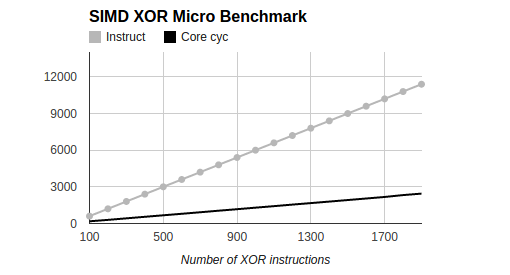
\includegraphics[width=140mm]{draw/testp_xor.png}
\caption[Test Performance with XOR]{Test performance with XOR\@. The dotted line is instruction count and the other line is core CPU cycles.}
\label{figure:testp_xor}
\end{figure}

From the figure, we can see the instruction count and CPU cycles grows linearly with the number of XOR instructions. So we can conclude that Fog's test program can be used to compare two pieces of critical code: the one with more measured CPU cycles is more complex and has more instructions. Note that from the figure, it seems the throughput of $xorps$ is 4, which is different from Intel's document (3.0 in document). We found this may be related to the compiler optimization on the loop; when we flattened the loop we got the throughput around 2.7. In order to eliminate this undesired effect, we flatten all the test code in the following sections.

In the following sections, we write micro benchmarks with Agner Fog's test program and compare performance between different implementation. Our test machine is X86 64-bit Ubuntu with Intel Haswell, and the detailed configuration can be found in Table~\ref{table:hardware_config}. In order to inline pure IR functions (instead of a function call into one object file), we compile all the test code into LLVM bit code (binary form of LLVM IR) and then link / optimize them together. The default compile flag is to use Intel SSE2 instruction set on the 64-bit OS.

\begin{table}[h]
\centering
\begin{tabular}{|c|c|}
\hline
CPU Name       & Intel(R) Core(TM) i5-4570 CPU \\ \hline
CPU MHz        & 3200                          \\ \hline
FPU            & Yes                           \\ \hline
CPU(s) enabled & 4 cores                       \\ \hline
L1 Cache       & 32 KB D + 32KB I              \\ \hline
L2 Cache       & 256 KB                        \\ \hline
L3 Cache       & 6 MB                          \\ \hline
Memory         & 8GB                           \\ \hline
\end{tabular}
\caption{Hardware Configuration}
\label{table:hardware_config}
\end{table}

\begin{table}[h]
\centering
\begin{tabular}{|c|c|}
\hline
Operating System & Ubuntu (Linux X86-64)         \\ \hline
Compiler         & Clang 3.5-1ubuntu1, GCC 4.8.2 \\ \hline
LLVM             & LLVM 3.5                      \\ \hline
File System      & Ext4                          \\ \hline
\end{tabular}
\caption{Software Configuration}
\label{table:software_config}
\end{table}

\subsection{Performance Against IDISA}
We compare our lowering on pure IR functions with the IDISA Library \cite{hua_idisa} which is written in C++. To test each operation, we generate a sequence of 500 such operations where none them has to wait for the previous one. 100 operations which are suggested by Agner seems too short for a stable result. This test sequence is generated by a template file.

For completeness, we choose all the operations listed in Table~\ref{table:semantics} except: NE (not equal), because IDISA does not support this operation; arbitrary shifts (SRL, SRA, SHL) because IDISA only supports immediate shifts; bitwise-logic (AND, OR, XOR), because the underline implementation are exactly the same and as simple as one line of machine code; we remove them to simplify the test code. Finally, we get eight operations for the micro-benchmark: ADD, SUB, MULT, EQ, LT, GT, ULT and UGT.

The performance comparison is listed in Figure~\ref{figure:cpu_cycles_vector} and Figure~\ref{figure:throughput_vector}. From Figure~\ref{figure:cpu_cycles_vector}, we can see for $i1$ and $i4$ vectors, the IR library has the similar CPU cycles with IDISA but it performs better with $i2$ vectors, especially on integer comparison.

The underlying logic for both libraries is the same, but it is implemented in different levels. For the IDISA library, {\tt simd<2>::ugt} is inline-extended immediately by the compiler front end and its semantics of integer comparison lost ever after, while in the IR library, for the whole life cycle before the instruction selection, {\tt ugt\_2} keeps its semantics. The extension of {\tt ugt\_2} is delayed until the instruction selection phase, right before machine code generation. And the delayed extension may help the compiler optimize as we discussed in Chapter~\ref{three}. We checked that the IDISA function {\tt simd<2>::ugt} and IR function {\tt ugt\_2} (whose underlying code is just \verb|icmp ugt <64 x i2> %a, %b|) generated different assembly code.

\begin{figure}[htbp!]
\centering
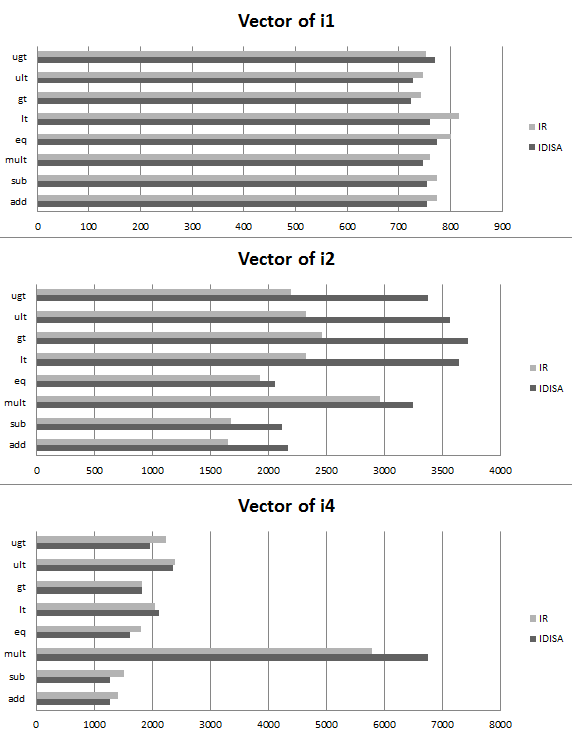
\includegraphics[width=140mm]{draw/cpu_cycles_vector.png}
\caption[Total CPU cycles against IDISA library]{Total CPU cycles against IDISA library; for $i1$ and $i4$ vectors, IR library has the similar performance with IDISA but it performs better with $i2$ vectors, especially on integer comparison.}
\label{figure:cpu_cycles_vector}
\end{figure}

\begin{figure}[htbp!]
\centering
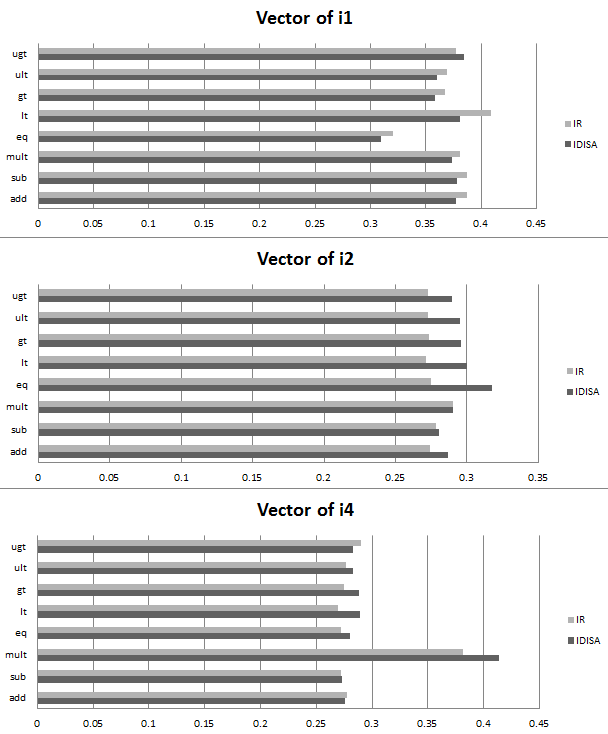
\includegraphics[width=140mm]{draw/reciprocal_throughput_vector.png}
\caption[Reciprocal instruction throughput against IDISA library]{Reciprocal instruction throughput against IDISA library. IR and IDISA share almost identical throughput.}
\label{figure:throughput_vector}
\end{figure}

However, the delay in expansion is not always good. Take multiplication on the $i2$ vector for an example, we can see our IR library has slightly bettered total CPU cycles, but if we write our instructions sequence with a loop, IDISA library wins (Figure~\ref{figure:loop_vector_i2}). Loop optimization is responsible for this difference; we did observe lines of assembly code hoisted outside the loop. Because all the operations tested here take two operands and the same constant value is used for all the second operand for simplicity, there is duplicated logic in each loop iteration that can be hoisted and shared. Hoisting was not done with the IR library. So early expansion in IDISA provides some optimization opportunity to the compiler.

From the reciprocal throughput comparison (Figure~\ref{figure:throughput_vector}), the IR library loses on $i1$ vectors but wins most of the cases in $i2$ and $i4$; it relates to a better instruction selection. IDISA library is generated from a strategy pool based on the number of machine instructions which are treated equally with cost 1. But machine instructions actually have different throughput in the real hardware, and the LLVM back end has more knowledge of that, thus selecting better instructions.

\begin{figure}[htbp!]
\centering
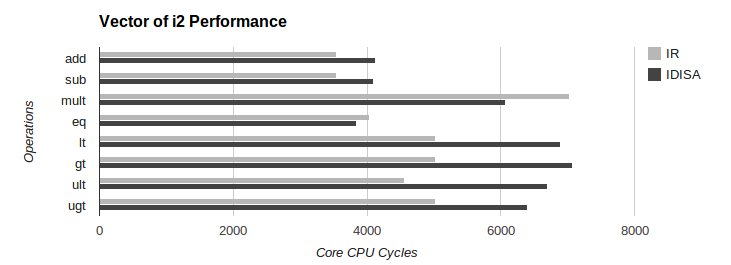
\includegraphics[width=140mm]{draw/loop_vector_i2.png}
\caption[Vector of $i2$ tested in a loop]{The same benchmark for $i2$ vectors with the instruction in a loop. Code in Figure~\ref{figure:cpu_cycles_vector} can be seen as the flattened version of this figure. We find IDISA here wins in the multiplication on $i2$, while IR wins it in Figure~\ref{figure:cpu_cycles_vector}. Loop optimization should be responsible for it.}
\label{figure:loop_vector_i2}
\end{figure}

\subsection{Performance Against LLVM}
We compare our lowering with native LLVM\@. LLVM could not handle $i2$, $i4$ vectors but could handle $i1$ vectors slowly. Detailed performance data can be found in Table~\ref{table:vector_perf_LLVM}. We can see that our approach fills the gap of the LLVM type system.

\begin{table}[h]
\centering
\begin{tabular}{|c|c|c|c|c|}
\hline
     & $i1$ & $i2$ & $i4$ & $i8$ \\ \hline
add  & 302  & X    & X    & 1\\ \hline
sub  & 310  & X    & X    & 1\\ \hline
mult & X    & X    & X    & 10\\ \hline
eq   & 273  & X    & X    & 1\\ \hline
lt   & X    & X    & X    & 1\\ \hline
gt   & X    & X    & X    & 1\\ \hline
ult  & 349  & X    & X    & 1\\ \hline
ugt  & 290  & X    & X    & 1\\ \hline
\end{tabular}
\caption[Performance against LLVM native support for $i2^k$ vectors]{Performance against LLVM native support of $i2^k$ vectors. `X' means compile error or compile too slowly (longer than 30s), the remaining number means the ratio of CPU cycles speed up: add takes 302 times of cycles that our lowering needs. For $i8$, we apply the inductive doubling strategy on the multiplication, which explains the 10 times speed up. }
\label{table:vector_perf_LLVM}
\end{table}

\section{Parabix Critical Operations}
In this section, we evaluate our work by replacing Parabix critical operations with the IR library. We first choose transposition and inverse transposition as two representative operations and then measure performance in two Parabix applications: XML validator and UTF-8 to UTF-16 transcoder. Note that we did not rewrite the whole application with an IR library, part of the application is still IDISA but some critical operations are replaced. The default compile flag is to use the Intel SSE2 instruction set on a 64-bit OS.

To compare performance, we use the same data files used in \cite{rob_xml}. The description of these files can be found in Table~\ref{table:xmlwf_data}.

\begin{table}[h]
\centering
\begin{tabular}{|c|c|c|c|c|c|}
\hline
File Name           & dew.xml & jaw.xml & roads-2.gml & po.xml  & soap.xml \\ \hline
File Type           & document   & document   & data      & data    & data     \\ \hline
File Size (MB)      & 66      & 7       & 11    & 76   & 3     \\ \hline
Markup Item Count   & 406k     & 74k      & 280k    & 4634k & 18k    \\ \hline
Attribute Count     & 18k      & 3k       & 160k    & 463k  & 30k    \\ \hline
Avg. Attribute Size & 8          & 8          & 6         & 5       & 9        \\ \hline
Markup Density      & 0.07       & 0.13       & 0.57      & 0.76    & 0.87     \\ \hline
\end{tabular}
\caption{XML Document Characteristics. Taken from \cite{rob_xml}.}
\label{table:xmlwf_data}
\end{table}

\begin{table}[h]
\centering
\begin{tabular}{|c|c|c|c|c|c|}
\hline
        & dew.xml  &  jaw.xml  &  roads-2.gml  &  po.xml  & soap.xml¬ \\\hline
xmlwf0   &  3.93   &    4.36   &   4.55   &   4.89   &   5.18 \\ \hline
xmlwf0 on Haswell   &  3.92   &   4.36   &   4.55   &   4.87   &   5.17 \\ \hline

xmlwf1   &  3.92   &   4.37   &   4.56   &   4.86   &   5.18 \\ \hline
xmlwf1 on Haswell &   3.56   &   3.97   &   4.16   &   4.45   &   4.78 \\ \hline
\end{tabular}
\caption[Performance comparison of XML Validator (xmlwf)]{Performance comparison of XML validator (xmlwf), in a thousand CPU cycles per thousand byte. In the table, xmlwf0 is implemented with full IDISA library and xmlwf1 is a copy of xmlwf0 with the transposition replaced.}
\label{table:xmlwf_perf}
\end{table}

\begin{table}[h]
\centering
\begin{tabular}{|c|c|c|c|c|c|}
\hline
 & dew.xml & jaw.xml & roads-2.gml & po.xml & soap.xml \\ \hline
 U8u16\_0         & 281.46  & 37.11   & 40.06       & 244.94 & 10.20    \\ \hline
 U8u16\_0 Haswell & 272.68  & 34.21   & 39.84       & 242.56 & 10.11    \\ \hline
 U8u16\_1         & 284.17  & 36.71   & 41.65       & 255.57 & 10.60     \\ \hline
 U8u16\_1 Haswell & 267.14  & 34.64   & 38.53       & 237.66 & 9.98     \\ \hline
 \end{tabular}
 \caption[Performance comparison of UTF-8 UTF-16 Transcoder]{Performance comparison of UTF-8 UTF-16 transcoder, in a million CPU cycles. U8u16\_0 is written in IDISA, U8u16\_1 has the transposition and inverse transposition part replaced.}
 \label{table:u8u16_perf}
 \end{table}

Table~\ref{table:xmlwf_perf} shows the performance of the XML Validator. The only difference of xmlwf0 and xmlwf1 is their transposition code. The one in xmlwf1 is written in pure IR with the byte-pack algorithm (the source code can be found in Appendix~\ref{appone:transposition}). We can see xmlwf0 and xmlwf1 share almost identical performance. LLVM 3.5 cannot handle packing on 16-bit field width very well so we custom lower the shufflevector and generate PACKUS instructions for X86 to get this good performance.

Another interesting observation is, when we re-compiled the same code on the Intel Haswell platform, we got almost no improvement for xmlwf0, since the IDISA library linked in is written with direct SSE2 intrinsic so only SSE2 instructions can be generated. But we got a slightly better performance for xmlwf1, because the IR library is target-independent. LLVM back end knows AVX2 is available so it generates VEX prefixed operations with three-operand form.

Similar performance data on the UTF-8 to UTF-16 transcoder is listed in Table~\ref{table:u8u16_perf}. U8u16\_0 is written in IDISA and U8u16\_1 has both the transposition and inverse transposition part replaced. Since our modified LLVM could not generate machine code for inverse transposition as good as IDISA, there are performance drops from U8u16\_0 to U8u16\_1. We also tried to compile them on the full Haswell, which gave us similar performance benefit from using AVX2 VEX operations. The feature of being target-independent helps Parabix to enjoy the improvement of hardware without changing its source code.

\subsection{Ideal 3-Stage Transposition on the Intel Haswell}
Intel Haswell architecture introduces the PEXT operation which can be used for the ideal 3-stage transposition (source code in Appendix~\ref{appone:transposition_ideal}). We evaluated its performance in Table~\ref{table:PEXT_transposition}. The performance dropped with PEXT, but the major reason is that PEXT can only work on $i32$ or $i64$ integers for the current architecture. As the hardware evolves, we may have PEXT on SIMD registers directly. At that time, we can expect a better performance in xmlwf2, may be better than both xmlwf0 and xmlwf1 since 3-stage transposition is proved to be optimal under the IDISA model \cite{inductive_doubling_principle}. Our approach provides a new chance to exploit future hardware improvements.

\begin{table}[h]
\centering
\begin{tabular}{|c|c|c|c|c|c|}
\hline
        & dew.xml  &  jaw.xml  &  roads-2.gml  &  po.xml  & soap.xml¬ \\\hline
xmlwf0 on Haswell   &  3.92   &   4.36   &   4.55   &   4.87   &   5.17 \\ \hline
xmlwf1 on Haswell &   3.56   &   3.98   &   4.16   &   4.45   &   4.78 \\ \hline
xmlwf2 on Haswell & 4.11   &    4.49   &    4.69   &    4.97   &   5.30 \\ \hline
\end{tabular}
\caption[Ideal 3-Stage Transposition with PEXT]{Performance of the ideal 3-stage transposition in a thousand CPU cycles per thousand byte. Xmlwf2 uses the ideal 3-stage transposition algorithm. Xmlwf1 uses byte-pack algorithm in IR, xmlwf0 uses the same algorithm in IDISA.}
\label{table:PEXT_transposition}
\end{table}

\subsection{Long Stream Addition And Shift}
We replaced the internal logic of big integer addition in Chapter~\ref{four} and introduced a new intrinsic: {\tt uadd.with.overflow.carryin}. We evaluate them in this section by first comparing the long-stream addition algorithm with LLVM's original implementation and then some application level profiles for the new intrinsic.

We wrote micro benchmarks with Fog's test program. We put 200 independent additions on $i128$ and $i256$. We choose 200 because 200 is a small number that can give us stable performance results. It was tricky to make the test program right; we generated random data for the operands and carefully inserted the carry-out bit back to the return value so that LLVM knows to use the long-stream-addition logic. In order to be consistent throughout the comparison, we used the same compiler flag for all the runs ({\tt -mavx2} for gcc and {\tt -mattr=+avx2,+bmi2} for LLVM tool chain). The result is listed in Table~\ref{table:lsadd_micro}.

\begin{table}[h]
\centering
\begin{tabular}{|c|c|c|}
\hline
                             & Core CPU Cycles & Instructions \\ \hline
LLVM on $i128$                 & 1455            & 4199         \\ \hline
Long stream addition on $i128$ & 2416            & 6552         \\ \hline
LLVM on $i256$                 & 4234            & 9798         \\ \hline
Long stream addition on $i256$ & 2656            & 6959        \\ \hline
\end{tabular}
\caption{Micro benchmarks for long stream addition against LLVM's original implementation.}
\label{table:lsadd_micro}
\end{table}

Long stream addition does not perform well on $i128$. Since there are only two sequential additions involved (1 $addq$ and 1 $adcq$), parallel computing does not save much but introduces new complexity. However, on $i256$ long stream addition has much better performance than the sequential one which generates 1 $addq$ and 3 $adcq$. As the width of the operand doubles, the CPU cycles from LLVM increases to the rate of 2.91, while in the long stream addition, the rate is only 1.10. This is because the time complexity of our algorithm is independent of the operand size while the sequential one has the time complexity linear to the operand size. Our algorithm scales better when the width of SIMD registers grows. We can confidently predict that on the Intel AVX512, long stream addition on $i512$ would out-perform the sequential one significantly.

An important Parabix application is regular expression matching. A grep-like tool was written recently with bitwise data parallelism called `icgrep' \cite{dale_icgrep}. Icgrep uses LLVM just-in-time compiling facility to generate IR code on the fly according to the input regular expression. We use icgrep to evaluate our new intrinsic for long stream addition. Its signature is in Program~\ref{prog:uadd_carryin} and it is used for the "add with carry" logic in icgrep.

\begin{program}[htbp!]
\begin{verbatim}
  {i128, i1} @llvm.uadd.with.overflow.carryin.i128(i128 %a, i128 %b, i1 %carryin)
  ; return a pair of sum and carry-out bit
\end{verbatim}
\caption[Signature of {\tt uadd.with.overflow.carryin}]{Signature of {\tt uadd.with.overflow.carryin}.}
\label{prog:uadd_carryin}
\end{program}

To compare with the unmodified LLVM, we need to emulate this new intrinsic. LLVM supports {\tt uadd.with.overflow} which does not take the carry-in bit into account. The pseudo code for "add with carry" is listed in Program~\ref{prog:uadd}. Then we can compare our back end with the unmodified LLVM\@. The same regular expressions and data files are used in \cite{rob_regex}. Since we only care about the improvement between back ends, the details of the regular expressions are not important. We show the relative instructions count in Figure~\ref{fig:inst_count_long_add} and we get around 20 percent improvement. The experiment was done with 128-bit SIMD registers. Most of the improvement comes from the fact that our back end only requires one addition. We also measured the relative CPU cycles. There are around 10 percent reduction in CPU cycles with our new intrinsic, which implies that the sequential addition has higher throughput (instructions per cycle).

\begin{program}[htbp!]
\begin{verbatim}
  declare {i128, i1} @llvm.uadd.with.overflow.i128(i128 %a, i128 %b)
  ;return a pair of sum and carry-out bit

  {i128, i1} @add_with_carry(i128 %a, i128 %b, i1 %carryin) {
  entry:
    cin = zext %carryin to i128

    {s1, c1} = @llvm.uadd.with.overflow.i128(%a, %b)
    {sum, c2} = @llvm.uadd.with.overflow.i128(s1, cin)

    cout = or i1 c1, c2
    ret {sum, cout}
  }
\end{verbatim}
\caption[Pseudo code for "add with carry" logic in with unmodified LLVM]{Pseudo code for "add with carry" logic in with unmodified LLVM\@.}
\label{prog:uadd}
\end{program}

\begin{figure}[htbp!]
\centering
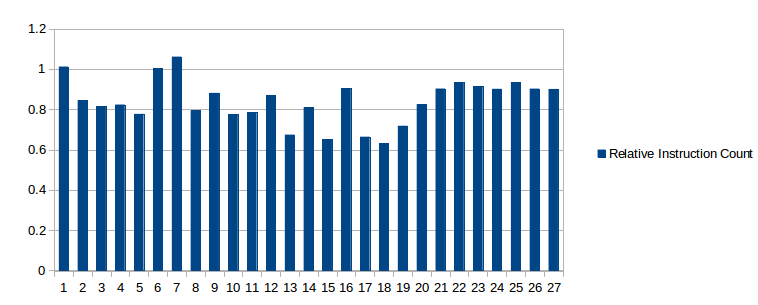
\includegraphics[width=140mm]{draw/inst_count_long_add.png}
\caption[Improvement with long stream addition and the new intrinsic in instruction count]{Improved instruction count with long stream addition. The number in the figure is the ratio of the instruction count in our back end to the count in unmodified LLVM. 27 pairs of regular expressions and data files are evaluated.}
\label{fig:inst_count_long_add}
\end{figure}

We then compare the long stream shifting algorithms. We discussed two algorithms in Section~\ref{sec:long_shift}; we implemented a DAG combiner in our back end. IR code of double shift can be compiled on the unmodified LLVM, so it is convenient that no new source code needs to be written. We used exactly the same code on both of the back ends. To avoid a difference in "add with carry", we used a logic that generates the same machine code on both back ends. The comparison of long stream shifting with 128-bit SIMD registers is listed in Figure~\ref{fig:inst_count_long_shift}. We can see a reduction of 10 to 20 percent in instructions. For CPU cycles, a reduction of 20 percent is achieved. The reduction in CPU cycles equals to, if not greater than, the reduction in instructions count. It means the long stream shifting uses less instructions as well as maintaining a good throughput.

\begin{figure}[htbp!]
\centering
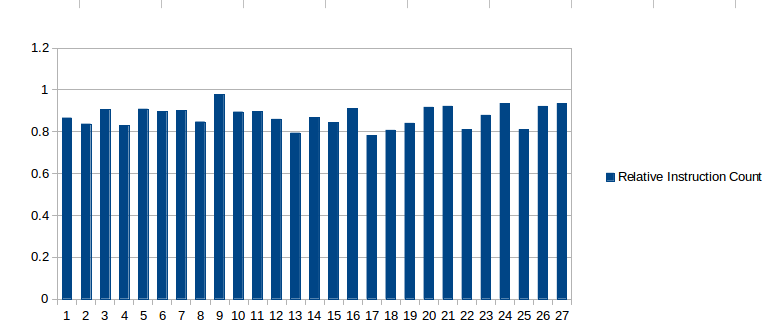
\includegraphics[width=140mm]{draw/inst_count_long_shift.png}
\caption[Improvement with long stream shifting in instruction count]{Improvement with long stream shifting in instruction count. The number in the figure is the ratio of the instruction count in our back end to the count in unmodified LLVM.}
\label{fig:inst_count_long_shift}
\end{figure}

Next, we study the behaviour of long stream addition and shifting with 256-bit SIMD registers. We turned on both of the optimizations for icgrep. The relative instruction count is listed in Figure~\ref{fig:inst_count_all_256}. From the micro-benchmark we already know that long stream addition works better than the sequential addition on this wider SIMD register. Together with long stream shifting, we achieved a substantial 30 to 40 percent instruction reduction against the unmodified LLVM\@. We also achieved around 40 percent reduction in CPU cycles.

\begin{figure}[htbp!]
\centering
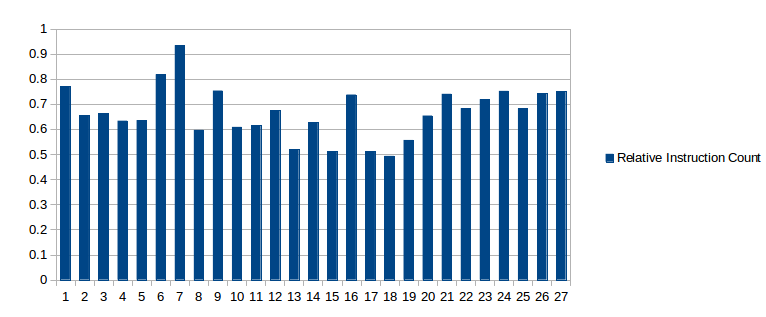
\includegraphics[width=140mm]{draw/inst_count_all_256.png}
\caption[Improvement of icgrep on machines with 256-bit SIMD registers]{Improvement of icgrep on machines with 256-bit SIMD registers. Both long stream shifting and addition are used. The instruction count is compared with the unmodified LLVM with 256-bit SIMD registers.}
\label{fig:inst_count_all_256}
\end{figure}

\begin{figure}[htbp!]
\centering
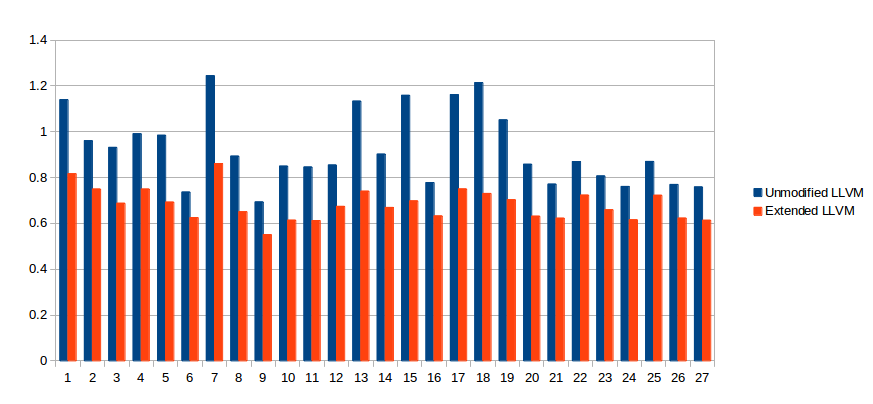
\includegraphics[width=140mm]{draw/inst_count_scalability.png}
\caption[Improved scalability of icgrep]{Improved scalability of icgrep. With the modified LLVM, icgrep gets more instructions count improvement by switching from 128-bit SIMD to 256-bit SIMD registers. Both long stream addition and shifting are used.}
\label{fig:inst_count_scalability}
\end{figure}

\begin{figure}[htbp!]
\centering
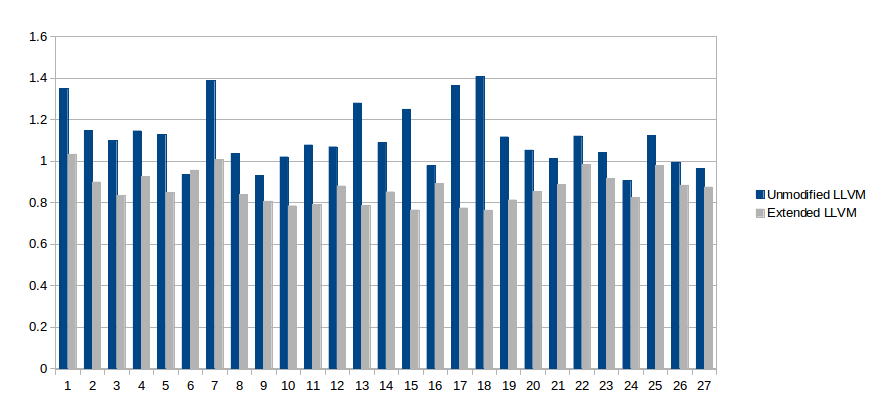
\includegraphics[width=140mm]{draw/cpu_cycles_scalability.png}
\caption[Improved scalability of icgrep in CPU cycles]{Improved scalability of icgrep in CPU cycles.}
\label{fig:cpu_cycles_scalability}
\end{figure}

Finally, we study the scalability of the modified LLVM\@. We want to check the improvement we can get by switching from 128-bit SIMD to 256-bit SIMD programming. We show the relative instructions count in Figure~\ref{fig:inst_count_scalability}. Extended LLVM can always benefit around 30 percent from using the wider SIMD registers, but the original LLVM sometimes even has performance drops. Figure~\ref{fig:cpu_cycles_scalability} shows the same comparison on a different metric: CPU cycles. Extended LLVM benefit around 20 percent from the wider SIMD registers. So we conclude that our LLVM back end has better scalability.
